\documentclass[9pt]{report}
%\usepackage[utopia]{mathdesign} 

\usepackage{amsmath,amsfonts,amsthm,amssymb,mathtools}
%\usepackage{amsmath,amsthm,mathtools}
\usepackage[french]{babel}
%\usepackage[utopia]{mathdesign}

% Permet d'ajuster la taille des marges et de la distance pour les footer
\usepackage[tmargin=2cm,rmargin=0.4in,lmargin=0.4in,bmargin=2cm,footskip=.2in]{geometry}

% Permet d'optimiser l'affichage de différents symboles et formules mathématiques
%\usepackage{amsmath,amsthm,mathtools}
%usepackage{amsmath,amsfonts,amsthm,amssymb,mathtools}

\usepackage{svg}
% Modifie l'apparence des nombre en mathmode et textmode
%\usepackage[varbb]{newpxmath}

% Modifier l'apparence des fractions
\usepackage{xfrac}

            %%%%%%%%%%%%%%%%%  Sect.        14 Oct 2024     %%%%%%%%%%%%%%%%%%%%%%%%%%%%%%%%%%%%%%%%%%%%%%%%%%%%%%%%%%%
\usepackage{graphicx}
\usepackage{caption}
\usepackage{subcaption}
\usepackage{arydshln}
            %%%%%%%%%%%%%%%%%  Sect.        14 Oct 2024     %%%%%%%%%%%%%%%%%%%%%%%%%%%%%%%%%%%%%%%%%%%%%%%%%%%%%%%%%%
\usepackage{balance}
\usepackage{dirtree}
\usepackage{titlesec}






% Permet de rayer (barrer) l'argument avec la touche
% \cancel{} \bcancel{} ou \xcancel{}
\usepackage[makeroom]{cancel}

% Extension du package amsmath; corrige certains bugs et déficiences de son prédecesseur
%\usepackage{mathtools}

% This package provides most of the flexibility you may want to customize the three basic list
% environments (enumerate, itemize and description)
\usepackage{bookmark} 

% Réorganiser les théorèmes et Lemmes. Usage complexe. 
% Référence : https://ctan.math.illinois.edu/macros/latex/contrib/theoremref/theoremref-doc.pdf
\hypersetup{hidelinks}
\usepackage{hyperref,theoremref} 

% Fournit un environnement pour créer des boîtes colorées
\usepackage[most,many,breakable]{tcolorbox}


%\newcommand\mycommfont[1]{\footnotesize\ttfamily\textcolor{blue}{#1}}\SetCommentSty{mycommfont}

%\newcommand{\incfig}[1]{%\def\svgwidth{\columnwidth}\import{./figures/}{#1.pdf_tex}}
\newcommand{\arc}[1]{\wideparen{#1}}

%Pour colorer les lignes séparatrices de tableaux
\usepackage{colortbl}
\usepackage{tikzsymbols}

\usepackage{framed}
\usepackage{titletoc}
\usepackage{etoolbox}
\usepackage{tabularx}
\usepackage{enumitem}
\usepackage{amsthm}
            %%%%%%%%%%%%%%%%%  Sect.        14 Oct 2024     %%%%%%%%%%%%%%%%%%%%%%%%%%%%%%%%%%%%%%%%%%%%%%%%%%%%%%%%%%%

\usepackage{lipsum}
\usepackage{titling}
\renewcommand\maketitlehooka{\null\mbox{}\vfill}
\renewcommand\maketitlehookd{\vfill\null}

\newcommand{\varitem}[3][black]{%
  \item[%
   \colorbox{#2}{\textcolor{#1}{\makebox(5.5,7){#3}}}%
  ]
}
\usepackage{afterpage}
\newcommand\myemptypage{
    \null
    \thispagestyle{empty}
    \addtocounter{page}{-1}
    \newpage
    }




% from https://tex.stackexchange.com/a/167024/121799
\newcommand{\ClaudioList}{red,DarkOrange1,Goldenrod1,Green3,blue!50!cyan,DarkOrchid2}
\newcommand{\SebastianoItem}[1]{\foreach \X[count=\Y] in \ClaudioList
{\ifnum\Y=#1\relax
\xdef\SebastianoColor{\X}
\fi
}
\tikz[baseline=(SebastianoItem.base),remember
picture]{%
\node[fill=\SebastianoColor,inner sep=4pt,font=\sffamily,fill opacity=0.5] (SebastianoItem){#1)};}
}
\newcommand{\SebastianoHighlight}{\tikz[overlay,remember picture]{%
\fill[\SebastianoColor,fill opacity=0.5] ([yshift=4pt,xshift=-\pgflinewidth]SebastianoItem.east) -- ++(4pt,-4pt)
-- ++(-4pt,-4pt) -- cycle;
}}   
            %%%%%%%%%%%%%%%%%  Sect.        14 Oct 2024     %%%%%%%%%%%%%%%%%%%%%%%%%%%%%%%%%%%%%%%%%%%%%%%%%%%%%%%%%%%





%====================================================================

%====================================================================
\newcommand*{\authorimg}[1]%
    { \raisebox{-1\baselineskip}{\includegraphics[width=\imagesize]{#1}}}
\newlength\imagesize  

\usepackage{pgfplots}
\pgfplotsset{compat=1.17}

%==========================================================================================
\usepackage{libris} 
\usepackage{etoolbox}
\usepackage[export]{adjustbox}% for positioning figures

\makeatletter
% Force le chapitre suivant sur la ligne succedant la fin du 
% chapitre précédent
\patchcmd{\chapter}{\if@openright\cleardoublepage\else\clearpage\fi}{}{}{}
\makeatother
\usepackage[Sonny]{fncychap}


%boîte de couleur grise
\tcbset{
  graybox/.style={
    colback=gray!20,
    colframe=black,
    sharp corners=downhill,
    boxrule=1pt,
    left=5pt,
    right=5pt,
    top=5pt,
    bottom=5pt,
    boxsep=0pt,
	 % <-- add four values for each corner
  }
}
\newtcolorbox{graybox}{graybox}

%==========================================================================================



\usepackage{xcolor}
\usepackage{varwidth}
\usepackage{varwidth}
\usepackage{etoolbox}
%\usepackage{authblk}
\usepackage{nameref}
\usepackage{multicol,array}
\usepackage{tikz-cd}
\usepackage[ruled,linesnumbered,ruled]{algorithm2e}
\usepackage{comment} % enables the use of multi-line comments (\ifx \fi) 
\usepackage{import}
\usepackage{xifthen}
\usepackage{pdfpages}
\usepackage{transparent}


%\usepackage[french]{babel}
\usepackage{listings} % pour écrire du code dans un environnement
\lstset{
  basicstyle=\ttfamily,
  columns=fullflexible,
  keepspaces=true
}
\usepackage{caption}
\usepackage{float} % Pour forcer les images au bon endroit



\usepackage[T1]{fontenc}
\usepackage{csquotes}
%%%%%%%%%%%%%%%%%%%%%%%%%%%%%%%%%%%%%%%%%%%%%%%%%%%%%%%%%%%%%%%%%%%%%%%%%%%%%%%%%%%%%%%%%%%%%%%%%
%									ENSEMBLE DE COULEURS
%%%%%%%%%%%%%%%%%%%%%%%%%%%%%%%%%%%%%%%%%%%%%%%%%%%%%%%%%%%%%%%%%%%%%%%%%%%%%%%%%%%%%%%%%%%%%%%%%

\definecolor{myg}{RGB}{56, 140, 70}
\definecolor{myb}{RGB}{45, 111, 177}

\definecolor{mygbg}{RGB}{235, 253, 241}


\definecolor{myr}{RGB}{199, 68, 64}
\definecolor{mytheorembg}{HTML}{F2F2F9}
\definecolor{mytheoremfr}{HTML}{00007B}
\definecolor{mylenmabg}{HTML}{FFFAF8}
\definecolor{mylenmafr}{HTML}{983b0f}
\definecolor{mypropbg}{HTML}{f2fbfc}
\definecolor{mypropfr}{HTML}{191971}
\definecolor{myexamplebg}{HTML}{F2FBF8}
\definecolor{myexamplefr}{HTML}{88D6D1}
\definecolor{myexampleti}{HTML}{2A7F7F}
\definecolor{mydefinitbg}{HTML}{E5E5FF}
\definecolor{mydefinitfr}{HTML}{3F3FA3}
\definecolor{notesgreen}{RGB}{0,162,0}
\definecolor{myp}{RGB}{197, 92, 212}
\definecolor{mygr}{HTML}{2C3338}
\definecolor{myred}{RGB}{127,0,0}
\definecolor{myyellow}{RGB}{169,121,69}
\definecolor{myexercisebg}{HTML}{F2FBF8}
\definecolor{myexercisefg}{HTML}{88D6D1}
\definecolor{myred}{RGB}{127,0,0}
\definecolor{myyellow}{RGB}{169,121,69}
\definecolor{LightLavender}{HTML}{DFC5FE}

\definecolor{blue}{HTML}{008ED7}
\definecolor{mygray}{gray}{0.75}
\definecolor{lightBlue}{RGB}{235, 245, 255}
\definecolor{tcbcolred}{RGB}{255,0,0}
\definecolor{myGreen}{HTML}{009900}

% command to circle a text
\newtcbox{\entoure}[1][red]{on line,
	arc=3pt,colback=#1!10!white,colframe=#1!50!black,
	before upper={\rule[-3pt]{0pt}{10pt}},boxrule=1pt,
	boxsep=0pt,left=2pt,right=2pt,top=1pt,bottom=.5pt}
% command for the circle for the number of part entries
\newcommand\Circle[1]{\tikz[overlay,remember picture]
	\node[draw,circle, text width=18pt,line width=1pt] {#1};}

\newtcbox{\entouree}[1][red]{on line,
	arc=3pt,colback=#1!10!white,colframe=#1!50!white,
	before upper={\rule[-3pt]{0pt}{10pt}},boxrule=1pt,
	boxsep=0pt,left=2pt,right=2pt,top=1pt,bottom=.5pt}

\newcommand{\shellcmd}[1]{\\\indent\indent\texttt{\footnotesize\# #1}\\}

%=====================================================================

\patchcmd{\tableofcontents}{\contentsname}{\rmfamily\contentsname}{}{}
% patching of \@part to typeset the part number inside a framed box in its own line
% and to add color
\makeatletter
\patchcmd{\@part}
  {\addcontentsline{toc}{part}{\thepart\hspace{1em}#1}}
  {\addtocontents{toc}{\protect\addvspace{20pt}}
    \addcontentsline{toc}{part}{\huge{\protect\color{myyellow}%
      \setlength\fboxrule{2pt}\protect\Circle{%
        \hfil\thepart\hfil%
      }%
    }\\[2ex]\color{myred}\rmfamily#1}}{}{}

%\patchcmd{\@part}
%  {\addcontentsline{toc}{part}{\thepart\hspace{1em}#1}}
%  {\addtocontents{toc}{\protect\addvspace{20pt}}
%    \addcontentsline{toc}{part}{\huge{\protect\color{myyellow}%
%      \setlength\fboxrule{2pt}\protect\fbox{\protect\parbox[c][1em][c]{1.5em}{%
%        \hfil\thepart\hfil%
%      }}%
%    }\\[2ex]\color{myred}\sffamily#1}}{}{}
\makeatother
% this is the environment used to typeset the chapter entries in the ToC
% it is a modification of the leftbar environment of the framed package
\renewenvironment{leftbar}
  {\def\FrameCommand{\hspace{6em}%
    {\color{myyellow}\vrule width 2pt depth 6pt}\hspace{1em}}%
    \MakeFramed{\parshape 1 0cm \dimexpr\textwidth-6em\relax\FrameRestore}\vskip2pt%
  }
 {\endMakeFramed}

% using titletoc we redefine the ToC entries for parts, chapters, sections, and subsections
\titlecontents{part}
  [0em]{\centering}
  {\contentslabel}
  {}{}
\titlecontents{chapter}
  [0em]{\vspace*{2\baselineskip}}
  {\parbox{4.5em}{%
    \hfill\Huge\rmfamily\bfseries\color{myred}\thecontentspage}%
   \vspace*{-2.3\baselineskip}\leftbar\textsc{\small\chaptername~\thecontentslabel}\\\rmfamily}
  {}{\endleftbar}
\titlecontents{section}
  [8.4em]
  {\rmfamily\contentslabel{3em}}{}{}
  {\hspace{0.5em}\nobreak\color{myred}\normalfont\contentspage}
\titlecontents{subsection}
  [8.4em]
  {\rmfamily\contentslabel{3em}}{}{}  
  {\hspace{0.5em}\nobreak\color{myred}\contentspage}


\tcbset{
  tbcsetLavender/.style={
    on line, 
    boxsep=4pt, left=0pt,right=0pt,top=0pt,bottom=0pt,
    colframe=white, colback=LightLavender,  
    highlight math style={enhanced}
  }
}
\tcbset{
  grayb/.style={
    on line, 
    boxsep=4pt, left=0pt,right=0pt,top=0pt,bottom=0pt,
    colframe=white, colback=gray!30,  
    highlight math style={enhanced}
  }
}


%==========================================================================

%PYTHON LSTLISTING STYLE

% Define colors
\definecolor{Pgruvbox-bg}{HTML}{282828}
\definecolor{Pgruvbox-fg}{HTML}{ebdbb2}
\definecolor{Pgruvbox-red}{HTML}{fb4934}
\definecolor{Pgruvbox-green}{HTML}{b8bb26}
\definecolor{Pgruvbox-yellow}{HTML}{fabd2f}
\definecolor{Pgruvbox-blue}{HTML}{83a598}
\definecolor{Pgruvbox-purple}{HTML}{d3869b}
\definecolor{Pgruvbox-aqua}{HTML}{8ec07c}

% Define Python style
\lstdefinestyle{PythonGruvbox}{
	language=Python,
	identifierstyle=\color{lst-fg},
	basicstyle=\ttfamily\color{Pgruvbox-fg},
	keywordstyle=\color{Pgruvbox-yellow},
	keywordstyle=[2]\color{Pgruvbox-blue},
	stringstyle=\color{Pgruvbox-green},
	commentstyle=\color{Pgruvbox-aqua},
	backgroundcolor=\color{Pgruvbox-bg},
	%frame=tb,
	rulecolor=\color{Pgruvbox-fg},
	showstringspaces=false,
	keepspaces=true,
	captionpos=b,
	breaklines=true,
	tabsize=4,
	showspaces=false,
	numbers=left,
	numbersep=5pt,
	numberstyle=\tiny\color{gray},
	showtabs=false,
	columns=fullflexible,
	morekeywords={True,False,None},
	morekeywords=[2]{and,as,assert,break,class,continue,def,del,elif,else,except,exec,finally,for,from,global,if,import,in,is,lambda,nonlocal,not,or,pass,print,raise,return,try,while,with,yield},
	morecomment=[s]{"""}{"""},
	morecomment=[s]{'''}{'''},
	morecomment=[l]{\#},
	morestring=[b]",
	morestring=[b]',
	literate=
	{0}{{\textcolor{Pgruvbox-purple}{0}}}{1}
	{1}{{\textcolor{Pgruvbox-purple}{1}}}{1}
	{2}{{\textcolor{Pgruvbox-purple}{2}}}{1}
	{3}{{\textcolor{Pgruvbox-purple}{3}}}{1}
	{4}{{\textcolor{Pgruvbox-purple}{4}}}{1}
	{5}{{\textcolor{Pgruvbox-purple}{5}}}{1}
	{6}{{\textcolor{Pgruvbox-purple}{6}}}{1}
	{7}{{\textcolor{Pgruvbox-purple}{7}}}{1}
	{8}{{\textcolor{Pgruvbox-purple}{8}}}{1}
	{9}{{\textcolor{Pgruvbox-purple}{9}}}{1}
}
%====================================================================
% 
%====================================================================

% JAVA LSTLISTING STYLE IN Gruvbox Colorscheme
\definecolor{gruvbox-bg}{rgb}{0.282, 0.247, 0.204}
\definecolor{gruvbox-fg1}{rgb}{0.949, 0.898, 0.776}
\definecolor{gruvbox-fg2}{rgb}{0.871, 0.804, 0.671}
\definecolor{gruvbox-red}{rgb}{0.788, 0.255, 0.259}
\definecolor{gruvbox-green}{rgb}{0.518, 0.604, 0.239}
\definecolor{gruvbox-yellow}{rgb}{0.914, 0.808, 0.427}
\definecolor{gruvbox-blue}{rgb}{0.353, 0.510, 0.784}
\definecolor{gruvbox-purple}{rgb}{0.576, 0.412, 0.659}
\definecolor{gruvbox-aqua}{rgb}{0.459, 0.631, 0.737}
\definecolor{gruvbox-gray}{rgb}{0.518, 0.494, 0.471}

\definecolor{lst-bg}{RGB}{45, 45, 45}
\definecolor{lst-fg}{RGB}{220, 220, 204}
\definecolor{lst-keyword}{RGB}{215, 186, 125}
\definecolor{lst-comment}{RGB}{117, 113, 94}
\definecolor{lst-string}{RGB}{163, 190, 140}
\definecolor{lst-number}{RGB}{181, 206, 168}
\definecolor{lst-type}{RGB}{218, 142, 130}


\lstdefinestyle{JavaGruvbox}{
	language=Java,
	basicstyle=\ttfamily\color{lst-fg},
	keywordstyle=\color{lst-keyword},
	keywordstyle=[2]\color{lst-type},
	commentstyle=\itshape\color{lst-comment},
	stringstyle=\color{lst-string},
	numberstyle=\color{lst-number},
	backgroundcolor=\color{lst-bg},
	%frame=tb,
	rulecolor=\color{gruvbox-aqua},
	showstringspaces=false,
	keepspaces=true,
	captionpos=b,
	breaklines=true,
	tabsize=4,
	showspaces=false,
	showtabs=false,
	columns=fullflexible,
	morekeywords={var},
	morekeywords=[2]{boolean, byte, char, double, float, int, long, short, void},
	morecomment=[s]{/}{/},
	morecomment=[l]{//},
	morestring=[b]",
	morestring=[b]',
	numbers=left,
	numbersep=5pt,
	numberstyle=\tiny\color{gray},
}



%====================================================================
% 
%====================================================================


% Define Dracula color scheme for Java
\definecolor{draculawhite-background}{RGB}{237, 239, 252}
\definecolor{draculawhite-comment}{RGB}{98, 114, 164}
\definecolor{draculawhite-keyword}{RGB}{189, 147, 249}
\definecolor{draculawhite-string}{RGB}{152, 195, 121}
\definecolor{draculawhite-number}{RGB}{249, 189, 89}
\definecolor{draculawhite-operator}{RGB}{248, 248, 242}

% Define JavaDraculaWhite lstlisting environment
\lstdefinestyle{JavaDraculaWhite}{
    language=Java,
    backgroundcolor=\color{draculawhite-background},
    commentstyle=\itshape\color{draculawhite-comment},
    keywordstyle=\ttfamily\color{draculawhite-keyword},
    stringstyle=\color{draculawhite-string},
    basicstyle=\ttfamily\footnotesize\color{black},
    identifierstyle=\color{myb!90},
    keywordstyle=\color{draculawhite-keyword}\bfseries,
    morecomment=[s][\color{draculawhite-comment}]{/**}{*/},
    showstringspaces=false,
    showspaces=false,
    breaklines=true,
    frame=single,
    rulecolor=\color{draculawhite-operator},
    tabsize=2,  
	numbers=left,
	numbersep=4pt,
	numberstyle=\ttfamily\tiny\color{gray}
}
%====================================================================
% 
%====================================================================
% Define PythonDraculaWhite lstlisting environment 
\definecolor{draculawhite-bg}{HTML}{FAFAFA}
\definecolor{draculawhite-fg}{HTML}{282A36}
\definecolor{pdraculawhite-keyword}{HTML}{BD93F9}

\definecolor{pdraculawhite-comment}{HTML}{6272A4}
\definecolor{draculawhite-number}{HTML}{FF79C6}


\lstdefinestyle{PythonDraculaWhite}{
    language=Python,
    basicstyle=\ttfamily\small\color{draculawhite-fg},
    backgroundcolor=\color{draculawhite-background},
    keywordstyle=\color{orange}\bfseries,
    stringstyle=\color{draculawhite-string},
    commentstyle=\color{pdraculawhite-comment}\itshape,
    numberstyle=\color{draculawhite-number},
    showstringspaces=false,
	showspaces=false,
    breaklines=true,
	frame=single,
	rulecolor=\color{draculawhite-operator}, 
    tabsize=4,
    morekeywords={as,with,1,2,3,4, 5,6,7,8,9,True,False},
    %escapeinside={(*@}{@*)},
    numbers=left,
    numbersep=5pt,
    %xleftmargin=15pt,
    %framexleftmargin=15pt,
    %framexrightmargin=0pt,
    %framexbottommargin=0pt,
    %framextopmargin=0pt,
    %rulecolor=\color{draculawhite-fg},
    %frame=tb,
    %aboveskip=0pt,
    %belowskip=0pt,
    %captionpos=b,
	numberstyle=\ttfamily\tiny\color{gray} 
}
%====================================================================
% 
%====================================================================

% Define colors for HTML langage
\definecolor{html-orange}{HTML}{FF5733}
\definecolor{html-yellow}{HTML}{F0E130}
\definecolor{html-green}{HTML}{50FA7B}
\definecolor{html-blue}{HTML}{5AFBFF}
\definecolor{html-purple}{HTML}{BD93F9}
\definecolor{html-pink}{HTML}{FF80BF}
\definecolor{html-gray}{HTML}{6272A4}
\definecolor{html-white}{HTML}{F8F8F2}

% Defines a new HTML5 langage that extend on the html langange
\lstdefinestyle{HTMLDraculaWhite}{
  language=HTML,
  backgroundcolor=\color{html-white},
  basicstyle=\ttfamily\color{html-gray},
  keywordstyle=\color{html-blue},
  stringstyle=\color{html-orange},
  commentstyle=\color{html-green},
  tagstyle=\color{html-yellow},
  moredelim=[s][\color{html-pink}]{<!--}{-->},
  moredelim=[s][\color{html-purple}]{\{}{\}},
  showstringspaces=false,
  tabsize=2,
  breaklines=true,
  columns=fullflexible,
  %frame=single,
  framexleftmargin=5mm,
  xleftmargin=10mm,
  numbers=left,
  numberstyle=\tiny\color{html-gray},
  escapeinside={<@}{@>}
}

%====================================================================
% 
%====================================================================
% Define the colors needed for the HTMLDraculaDark environment
\definecolor{htmltag}{HTML}{ff79c6}
\definecolor{htmlattr}{HTML}{f1fa8c}
\definecolor{htmlvalue}{HTML}{bd93f9}
\definecolor{htmlcomment}{HTML}{6272a4}
%\definecolor{htmltext}{HTML}{f8f8f2}
\definecolor{htmltext}{HTML}{401E31}
\definecolor{htmlbackground}{HTML}{282a36}
\definecolor{comphtmlbackground}{HTML}{8093FF}
%\definecolor{htmlbackground}{HTML}{4D5169}

% Define the HTMLDraculaDark environment
\lstdefinestyle{HTMLDraculaDark}{
    basicstyle=\bfseries\ttfamily\color{htmltext},
    commentstyle=\itshape\color{htmlcomment},
    keywordstyle=\bfseries\color{htmltag},
    stringstyle=\color{htmlvalue},
    emph={DOCTYPE,html,head,body,div,span,a,script},
    emphstyle={\color{htmltag}\bfseries},
    sensitive=true,
    showstringspaces=false,
    backgroundcolor=\color{white},
    %frame=tb,
    language=HTML,
    tabsize=4,
    breaklines=true,
    breakatwhitespace=true,
    numbers=left,
    numbersep=10pt,
    numberstyle=\small\bfseries\ttfamily\color{htmlcomment},
    escapeinside={<@}{@>},
	rulecolor=\color{htmlbackground},
	xleftmargin=20pt,
	% Add a vertical line for opening and closing tags
    %frame=lines,
    framesep=2pt,
    framexleftmargin=4pt,
    % Add a vertical line for closing tags that go through multiple lines
    breaklines=true,
    postbreak=\mbox{\textcolor{gray}{$\hookrightarrow$}\space},
    showlines=true,
	% Add a rule to apply commentstyle to keywords inside comments
    moredelim=[s][\itshape\color{htmlcomment}]{<!--}{-->},
    morekeywords={id,class,type,name,value,placeholder,checked,src,href,alt}
}




%====================================================================
% 
%====================================================================






% Crée un environnement "Theorem" numéroté en fonction du document
\tcbuselibrary{theorems,skins,hooks} 
\newtcbtheorem{Theorem}{Théorème}
{%
	enhanced,
	breakable,
	colback = mytheorembg,
	frame hidden,
	boxrule = 0sp,
	borderline west = {2pt}{0pt}{mytheoremfr},
	sharp corners,
	detach title,
	before upper = \tcbtitle\par\smallskip,
	coltitle = mytheoremfr,
	fonttitle = \bfseries\fontfamily{lmss}\selectfont,
	description font = \mdseries\fontfamily{lmss}\selectfont,
	separator sign none,
	segmentation style={solid, mytheoremfr},
}
{thm}

% Crée un environnement "Preuve" numéroté en fonction du document
\tcbuselibrary{theorems,skins,hooks}
\newtcbtheorem{Preuve}{Preuve}
{
	enhanced,
	breakable,
	colback=white,
	frame hidden,
	boxrule = 0sp,
	borderline west = {2pt}{0pt}{mytheoremfr},
	sharp corners,
	detach title,
	before upper = \tcbtitle\par\smallskip,
	coltitle = mytheoremfr,
	description font=\fontfamily{lmss}\selectfont,
	fonttitle=\fontfamily{lmss}\selectfont\bfseries,
	separator sign none,
	segmentation style={solid, mytheoremfr},
}
{th}


% Crée un environnement "Preuve" numéroté en fonction du document
\tcbuselibrary{theorems,skins,hooks}
\newtcbtheorem{Explication}{Explication}
{
	enhanced,
	breakable,
	colback=white,
	frame hidden,
	boxrule = 0sp,
	borderline west = {2pt}{0pt}{mytheoremfr},
	sharp corners,
	detach title,
	before upper = \tcbtitle\par\smallskip,
	coltitle = mytheoremfr,
	description font=\fontfamily{lmss}\selectfont,
	fonttitle=\fontfamily{lmss}\selectfont\bfseries,
	separator sign none,
	segmentation style={solid, mytheoremfr},
}
{th}




% Crée un environnement "Example" numéroté en fonction du document
\tcbuselibrary{theorems,skins,hooks}
\newtcbtheorem{Example}{Exemple.}
{
	enhanced,
	breakable,
	colback=lightBlue,
	frame hidden,
	boxrule = 0sp,
	borderline west = {2pt}{0pt}{myb},
	sharp corners,
	detach title,
	before upper = \tcbtitle\par\smallskip,
	coltitle = myb,
	description font=\fontfamily{lmss}\selectfont,
	fonttitle=\fontfamily{lmss}\selectfont\bfseries,
	separator sign none,
	segmentation style={solid, mytheoremfr},
}
{th}



% Crée un environnement "EExample" numéroté en fonction du document
\tcbuselibrary{theorems,skins,hooks}
\newtcbtheorem{EExample}{Exemple}
{
	enhanced,
	breakable,
	colback=white,
	frame hidden,
	boxrule = 0sp,
	borderline west = {2pt}{0pt}{myb},
	sharp corners,
	detach title,
	before upper = \tcbtitle\par\smallskip,
	coltitle = myb,
	description font=\mdseries\fontfamily{lmss}\selectfont,
	fonttitle=\fontfamily{lmss}\selectfont\bfseries,
	separator sign none,
	segmentation style={solid, mytheoremfr},
}
{th}



% Crée un environnement "Lemme" numéroté en fonction du document
\tcbuselibrary{theorems,skins,hooks}
\newtcbtheorem{Lemme}{Lemme}
{
	enhanced,
	breakable,
	colback=mylenmabg,
	frame hidden,
	boxrule = 0sp,
	borderline west = {2pt}{0pt}{mylenmafr},
	sharp corners,
	detach title,
	before upper = \tcbtitle\par\smallskip,
	coltitle = mylenmafr,
	description font=\mdseries\fontfamily{lmss}\selectfont,
	fonttitle=\fontfamily{lmss}\selectfont\bfseries,
	separator sign none,
	segmentation style={solid, mytheoremfr},
}
{th}


\tcbuselibrary{theorems,skins,hooks}
\newtcbtheorem{PreuveL}{Preuve.}
{
	enhanced,
	breakable,
	colback=white,
	frame hidden,
	boxrule = 0sp,
	borderline west = {2pt}{0pt}{mylenmafr},
	sharp corners,
	detach title,
	before upper = \tcbtitle\par\smallskip,
	coltitle = mylenmafr,
	description font=\fontfamily{lmss}\selectfont,
	fonttitle=\fontfamily{lmss}\selectfont\bfseries,
	separator sign none,
	segmentation style={solid, mytheoremfr},
}
{th}


\newtcbtheorem{Remarque}{Remarque}
{
	enhanced,
	breakable,
	colback=white,
	frame hidden,
	boxrule = 0sp,
	borderline west = {2pt}{0pt}{myb},
	sharp corners,
	detach title,
	before upper = \tcbtitle\par\smallskip,
	coltitle = myb,
	description font=\mdseries\fontfamily{lmss}\selectfont,
	fonttitle=\fontfamily{lmss}\selectfont\bfseries,
	separator sign none,
	segmentation style={solid, mytheoremfr},
}
{th}


\newtcbtheorem{DefG}{Définition}
{
	enhanced,
	breakable,
	colback=mygbg,
	frame hidden,
	boxrule = 0sp,
	borderline west = {2pt}{0pt}{myg},
	sharp corners,
	detach title,
	before upper = \tcbtitle\par\smallskip,
	coltitle = myg,
	description font=\mdseries\fontfamily{lmss}\selectfont,
	fonttitle=\fontfamily{lmss}\selectfont\bfseries,
	separator sign none,
	segmentation style={solid, mytheoremfr},
}
{th}



% Crée une boîte ayant la même couleur que l'environnement theorem.
\tcbuselibrary{theorems,skins,hooks}
\newtcolorbox{Theoremcon}
{%
	enhanced
	,breakable
	,colback = mytheorembg
	,frame hidden
	,boxrule = 0sp
	,borderline west = {2pt}{0pt}{mytheoremfr}
	,sharp corners
	,description font = \mdseries
	,separator sign none
}

% Crée un environnement "Definition" numéroté en fonction de la section
\newtcbtheorem[number within=chapter]{Definition}{Définition}{enhanced,
	before skip=2mm,after skip=2mm, colback=red!5,colframe=red!80!black,boxrule=0.5mm,
	attach boxed title to top left={xshift=1cm,yshift*=1mm-\tcboxedtitleheight}, varwidth boxed title*=-3cm,
	boxed title style={frame code={
			\path[fill=tcbcolback!10!red]
			([yshift=-1mm,xshift=-1mm]frame.north west)
			arc[start angle=0,end angle=180,radius=1mm]
			([yshift=-1mm,xshift=1mm]frame.north east)
			arc[start angle=180,end angle=0,radius=1mm];
			\path[left color=tcbcolback!10!myred,right color=tcbcolback!10!myred,
			middle color=tcbcolback!60!myred]
			([xshift=-2mm]frame.north west) -- ([xshift=2mm]frame.north east)
			[rounded corners=1mm]-- ([xshift=1mm,yshift=-1mm]frame.north east)
			-- (frame.south east) -- (frame.south west)
			-- ([xshift=-1mm,yshift=-1mm]frame.north west)
			[sharp corners]-- cycle;
		},interior engine=empty,
	},
	fonttitle=\bfseries,
	title={#2},#1}{def}

% Crée un environnement "definition" numéroté en fonction du Chapitre
\newtcbtheorem[number within=section]{definition}{Définition}{enhanced,
	before skip=2mm,after skip=2mm, colback=red!5,colframe=red!80!black,boxrule=0.5mm,
	attach boxed title to top left={xshift=1cm,yshift*=1mm-\tcboxedtitleheight}, varwidth boxed title*=-3cm,
	boxed title style={frame code={
			\path[fill=tcbcolback]
			([yshift=-1mm,xshift=-1mm]frame.north west)
			arc[start angle=0,end angle=180,radius=1mm]
			([yshift=-1mm,xshift=1mm]frame.north east)
			arc[start angle=180,end angle=0,radius=1mm];
			\path[left color=tcbcolback!60!black,right color=tcbcolback!60!black,
			middle color=tcbcolback!80!black]
			([xshift=-2mm]frame.north west) -- ([xshift=2mm]frame.north east)
			[rounded corners=1mm]-- ([xshift=1mm,yshift=-1mm]frame.north east)
			-- (frame.south east) -- (frame.south west)
			-- ([xshift=-1mm,yshift=-1mm]frame.north west)
			[sharp corners]-- cycle;
		},interior engine=empty,
	},
	fonttitle=\bfseries,
	title={#2},#1}{def}

\usetikzlibrary{arrows,calc,shadows.blur}
\tcbuselibrary{skins}
\newtcolorbox{note}[1][]{%
	enhanced jigsaw,
	colback=gray!20!white,%
	colframe=gray!80!black,
	size=small,
	boxrule=1pt,
	title=\textbf{Note : },
	halign title=flush center,
	coltitle=black,
	breakable,
	drop shadow=black!50!white,
	attach boxed title to top left={xshift=1cm,yshift=-\tcboxedtitleheight/2,yshifttext=-\tcboxedtitleheight/2},
	minipage boxed title=1.5cm,
	boxed title style={%
		colback=white,
		size=fbox,
		boxrule=1pt,
		boxsep=2pt,
		underlay={%
			\coordinate (dotA) at ($(interior.west) + (-0.5pt,0)$);
			\coordinate (dotB) at ($(interior.east) + (0.5pt,0)$);
			\begin{scope}
				\clip (interior.north west) rectangle ([xshift=3ex]interior.east);
				\filldraw [white, blur shadow={shadow opacity=60, shadow yshift=-.75ex}, rounded corners=2pt] (interior.north west) rectangle (interior.south east);
			\end{scope}
			\begin{scope}[gray!80!black]
				\fill (dotA) circle (2pt);
				\fill (dotB) circle (2pt);
			\end{scope}
		},
	},
	#1,
}


% Crée un environnement "qstion" 
\newtcbtheorem{qstion}{Question}{enhanced,
	breakable,
	colback=white,
	colframe=mygr,
	attach boxed title to top left={yshift*=-\tcboxedtitleheight},
	fonttitle=\bfseries,
	title={#2},
	boxed title size=title,
	boxed title style={%
		sharp corners,
		rounded corners=northwest,
		colback=tcbcolframe,
		boxrule=0pt,
	},
}{def}


% Pour créer un environnement "Liste" 

\tcbuselibrary{theorems,skins,hooks}
\newtcbtheorem[number within=section]{Liste}{Liste}
{%
	enhanced
	,breakable
	,colback = myp!10
	,frame hidden
	,boxrule = 0sp
	,borderline west = {2pt}{0pt}{myp!85!black}
	,sharp corners
	,detach title
	,before upper = \tcbtitle\par\smallskip
	,coltitle = myp!85!black
	,fonttitle = \bfseries\sffamily
	,description font = \mdseries
	,separator sign none
	,segmentation style={solid, myp!85!black}
}
{th}


\tcbuselibrary{theorems,skins,hooks}
\newtcbtheorem{Syntaxe}{Syntaxe.}
{%
	enhanced
	,breakable
	,colback = myp!10
	,frame hidden
	,boxrule = 0sp
	,borderline west = {2pt}{0pt}{myp!85!black}
	,sharp corners
	,detach title
	,before upper = \tcbtitle\par\smallskip
	,coltitle = myp!85!black
	,fonttitle = \bfseries\fontfamily{lmss}\selectfont 
	,description font = \mdseries\fontfamily{lmss}\selectfont 
	,separator sign none
	,segmentation style={solid, myp!85!black}
}
{th}



% Crée un environnement "Concept" numéroté en fonction du document
\tcbuselibrary{theorems,skins,hooks}
\newtcbtheorem{Concept}{Concept.}
{
	enhanced,
	breakable,
	colback=mylenmabg,
	frame hidden,
	boxrule = 0sp,
	borderline west = {2pt}{0pt}{mylenmafr},
	sharp corners,
	detach title,
	before upper = \tcbtitle\par\smallskip,
	coltitle = mylenmafr,
	description font=\mdseries\fontfamily{lmss}\selectfont,
	fonttitle=\fontfamily{lmss}\selectfont\bfseries,
	separator sign none,
	segmentation style={solid, mytheoremfr},
}
{th}


% Crée un environnement "codeEx" numéroté en fonction du document
\tcbuselibrary{theorems,skins,hooks}
\newtcbtheorem{codeEx}{Exemple}
{
	enhanced,
	breakable,
	colback=white,
	frame hidden,
	boxrule = 0sp,
	borderline west = {2pt}{0pt}{gruvbox-bg},
	sharp corners,
	detach title,
	before upper = \tcbtitle\par\smallskip,
	coltitle = gruvbox-bg,
	description font=\md:wqseries\fontfamily{lmss}\selectfont,
	fonttitle=\fontfamily{lmss}\selectfont\bfseries,
	separator sign none,
	segmentation style={solid, mytheoremfr},
}
{th}


% Crée un environnement "codeEx" numéroté en fonction du document
\tcbuselibrary{theorems,skins,hooks}
\newtcbtheorem{codeRem}{Remarque.}
{
	enhanced,
	breakable,
	colback=white,
	frame hidden,
	boxrule = 0sp,
	borderline west = {2pt}{0pt}{gruvbox-bg},
	sharp corners,
	detach title,
	before upper = \tcbtitle\par\smallskip,
	coltitle = gruvbox-bg,
	description font=\mdseries\fontfamily{lmss}\selectfont,
	fonttitle=\fontfamily{lmss}\selectfont\bfseries,
	separator sign none,
	segmentation style={solid, mytheoremfr},
}
{th}


\tcbuselibrary{theorems,skins,hooks}
\newtcbtheorem{Identite}{Identité.}
{
	enhanced,
	breakable,
	colback=white,
  before upper=\tcbtitle\par\Hugeskip,
	frame hidden,
	boxrule = 0sp,
	borderline west = {2pt}{0pt}{gruvbox-bg},
	sharp corners,
	detach title,
	before upper = \tcbtitle\par\smallskip,
	coltitle = gruvbox-bg,
	description font=\mdseries\fontfamily{lmss}\selectfont,
	fonttitle=\fontfamily{lmss}\selectfont\bfseries,
	fontlower=\fontfamily{cmr}\selectfont,
  separator sign none,
	segmentation style={solid, mytheoremfr},
}
{th}

\tcbuselibrary{theorems,skins,hooks}
\newtcbtheorem{Exercice}{Exercice}
{
	enhanced,
	breakable,
	colback=white,
  before upper=\tcbtitle\par\Hugeskip,
	frame hidden,
	boxrule = 0sp,
	borderline west = {2pt}{0pt}{gruvbox-green},
	sharp corners,
	detach title,
	before upper = \tcbtitle\par\smallskip,
	coltitle = gruvbox-green,
	description font=\mdseries\fontfamily{lmss}\selectfont,
	fonttitle=\fontfamily{lmss}\selectfont\bfseries,
	fontlower=\fontfamily{cmr}\selectfont,
  separator sign none,
	segmentation style={solid, mytheoremfr},
}
{th}

% Crée un environnement "Réponse" numéroté en fonction du document
\tcbuselibrary{theorems,skins,hooks}
\newtcbtheorem{Reponse}{Réponse}
{
	enhanced,
	breakable,
	colback=white,
	frame hidden,
	boxrule = 0sp,
	borderline west = {2pt}{0pt}{mytheoremfr},
	sharp corners,
	detach title,
	before upper = \tcbtitle\par\smallskip,
	coltitle = mytheoremfr,
	description font=\fontfamily{lmss}\selectfont,
	fonttitle=\fontfamily{lmss}\selectfont\bfseries,
	separator sign none,
	segmentation style={solid, mytheoremfr},
}
{th}

\newtcbtheorem{Definitionx}{Définition}
{
enhanced,
breakable,
colback=red!5,
  before upper=\tcbtitle\par\Hugeskip,
frame hidden,
boxrule = 0sp,
borderline west = {2pt}{0pt}{red!80!black},
sharp corners,
detach title,
before upper = \tcbtitle\par\smallskip,
coltitle = red!80!black,
description font=\mdseries\fontfamily{lmss}\selectfont,
fonttitle=\fontfamily{lmss}\selectfont\bfseries,
fontlower=\fontfamily{cmr}\selectfont,
  separator sign none,
segmentation style={solid, mytheoremfr},
}
{th}

\tcbuselibrary{theorems,skins,hooks}
\newtcbtheorem[number within=chapter]{prop}{Proposition}
{%
	enhanced,
	breakable,
	colback = mypropbg,
	frame hidden,
	boxrule = 0sp,
	borderline west = {2pt}{0pt}{mypropfr},
	sharp corners,
	detach title,
	before upper = \tcbtitle\par\smallskip,
	coltitle = mypropfr,
	fonttitle = \bfseries\sffamily,
	description font = \mdseries,
	separator sign none,
	segmentation style={solid, mypropfr},
}
{th}


\tcbuselibrary{theorems,skins,hooks}
\newtcbtheorem[number within=section]{Prop}{Proposition}
{%
	enhanced,
	breakable,
	colback = mypropbg,
	frame hidden,
	boxrule = 0sp,
	borderline west = {2pt}{0pt}{mypropfr},
	sharp corners,
	detach title,
	before upper = \tcbtitle\par\smallskip,
	coltitle = mypropfr,
	fonttitle = \bfseries\sffamily,
	description font = \mdseries,
	separator sign none,
	segmentation style={solid, mypropfr},
}
{th}


%================================
% Corollery
%================================
\tcbuselibrary{theorems,skins,hooks}
\newtcbtheorem[number within=section]{Corollary}{Corollary}
{%
	enhanced
	,breakable
	,colback = myp!10
	,frame hidden
	,boxrule = 0sp
	,borderline west = {2pt}{0pt}{myp!85!black}
	,sharp corners
	,detach title
	,before upper = \tcbtitle\par\smallskip
	,coltitle = myp!85!black
	,fonttitle = \bfseries\sffamily
	,description font = \mdseries
	,separator sign none
	,segmentation style={solid, myp!85!black}
}
{th}
\tcbuselibrary{theorems,skins,hooks}
\newtcbtheorem[number within=chapter]{corollary}{Corollaire}
{%
	enhanced
	,breakable
	,colback = myp!10
	,frame hidden
	,boxrule = 0sp
	,borderline west = {2pt}{0pt}{myp!85!black}
	,sharp corners
	,detach title
	,before upper = \tcbtitle\par\smallskip
	,coltitle = myp!85!black
	,fonttitle = \bfseries\sffamily
	,description font = \mdseries
	,separator sign none
	,segmentation style={solid, myp!85!black}
}
{th}



\usepackage[scr]{rsfso}

\usepackage{titlesec}
\usepackage{microtype}
\usepackage[utf8]{inputenc} % Required for inputting international characters
\usepackage[T1]{fontenc} % Output font encoding for international characters

\definecolor{myblue}{RGB}{0,82,155}


\lstset{basicstyle=\ttfamily}
%\usepackage[euler-digits]{eulervm}
\usepackage{mathpazo}
%\usepackage{palatino}
%usepackage{crimson}
\usepackage{libertine}


% Save the original definition of the mathpazo typewriter font
\newcommand{\mathpazott}{\fontfamily{pplj}\selectfont}

% Patch the \texttt command to use the mathpazo typewriter font
\let\oldtexttt\texttt
\renewcommand{\texttt}[1]{{\scriptsize\mathpazott #1}}


%\title{\Huge{Interface PM }\\{IFT2015}\\{\textbf{Devoir 1}}}
%\author{\huge{Franz Girardin}}
%\date{\today}
\newcommand{\plogo}{\fbox{$\mathcal{PL}$}} % Generic dummy publisher logo
\lstset{inputencoding=utf8/latin1}






            %%%%%%%%%%%%%%%%%  Sect.                          %%%%%%%%%%%%%%%%%%%%%%%%%%%%%%%%%%%%%%%%%%%%%%%%%%%%%%%%%
%\usepackage{helvet}
\titleformat{\chapter}[display]
  {\normalfont\bfseries\color{myblue}}
  {\filleft%
    \begin{tikzpicture}
    \node[
      outer sep=0pt,
      text width=1.5cm,
      minimum height=2cm,
      fill=myblue,
      font=\color{white}\fontsize{40}{50}\selectfont,
      align=center
      ] (num) {\thechapter};
    \node[
      rotate=90,
      anchor=south,
      font=\color{black}\Large\normalfont
      ] at ([xshift=-5pt]num.west) {\textls[180]{\textsc{Section}}};  
    \end{tikzpicture}%
  }
  {5pt}
  {\titlerule[2.0pt]\vskip3pt\titlerule\vskip4pt\LARGE\normalfont}

\titleformat{\section}
  {\normalfont\scshape}{\thesection}{1em}{}


% Customizing the spacing for the chapter titles
\titlespacing*{\chapter}{0pt}{0pt}{20pt}

% Allow hfill in math environment
\newcommand{\specialcell}[1]{\ifmeasuring@#1\else\omit$\displaystyle#1$\ignorespaces\fi}

% Allow you to do the non implication (implication barred)
\newcommand{\notimplies}{%
  \mathrel{{\ooalign{\hidewidth$\not\phantom{=}$\hidewidth\cr$\implies$}}}}



\DeclareRobustCommand{\looongrightarrow}{%
  \DOTSB\relbar\joinrel\relbar\joinrel\relbar\joinrel\rightarrow
}


\DeclareMathOperator{\di}{d\!}
\newcommand*\Eval[3]{\left.#1\right\rvert_{#2}^{#3}}

\begin{document}
\begin{titlepage} % Suppresses displaying the page number on the title page and the subsequent page counts as page 1
	\newcommand{\HRule}{\rule{\linewidth}{0.5mm}} % Defines a new command for horizontal lines, change thickness here
	
	\center % Centre everything on the page
	
	%------------------------------------------------
	%	Headings
	%------------------------------------------------
	
	\textsc{\LARGE Université de Montréal}\\[1.5cm] % Main heading such as the name of your university/college
	
	\textsc{\Large Département d'Informatique et de Recherche Opérationnelle}\\[0.5cm] % Major heading such as course name
	
	\textsc{\large Interface Prsonne-Machine}\\[0.5cm] % Minor heading such as course title
	
	%------------------------------------------------
	%	Title
	%------------------------------------------------
	
	\HRule\\[0.4cm]
	
	{\huge\bfseries Analyse de Design Web et Conception de Design Alternatif}\\[0.4cm] % Title of your document
	
	\HRule\\[1.5cm]
	
	%------------------------------------------------
	%	Author(s)
	%------------------------------------------------
	
	\begin{minipage}{0.4\textwidth}
		\begin{flushleft}
			\large
			\textit{Auteur}\\
		Franz \textsc{Girardin} \\ % Your name
		Nourdin \textsc{Azami} \\ 
    Emmanuel F. Gérald \textsc{Paraison} \\ % Your name
  	Martin \textsc{Medina} \\
    Étienne \textsc{Mitchell-Bouch}
		\end{flushleft}
	\end{minipage}
	~
	\begin{minipage}{0.4\textwidth}
		\begin{flushright}
			\large
			\textit{Matricule}\\
			\textsc{20078678} \\ % Supervisor's name
			\textsc{20202901} \\ 
      \textsc{20189461} \\% Supervisor's name
      \textsc{20235219} \\ 
      \textsc{20243430}
		\end{flushright}
	\end{minipage}
	
	% If you don't want a supervisor, uncomment the two lines below and comment the code above
	%{\large\textit{Author}}\\
	%John \textsc{Smith} % Your name
	
	%------------------------------------------------
	%	Date
	%------------------------------------------------
	
	\vfill\vfill\vfill % Position the date 3/4 down the remaining page
	
	{\large\today} % Date, change the \today to a set date if you want to be precise
	
	%------------------------------------------------
	%	Logo
	%------------------------------------------------
	
	%\vfill\vfill
	%\includegraphics[width=0.2\textwidth]{placeholder.jpg}\\[1cm] % Include a department/university logo - this will require the graphicx package
	 
	%----------------------------------------------------------------------------------------
	
	\vfill % Push the date up 1/4 of the remaining page
	
\end{titlepage}
\tableofcontents
\pagebreak



\begin{multicols*}{2}
  \small
\chapter{Scénario et présentation du site Web}



  \begin{Exercice}{(5 pts)}{}
  Choisissez un site Web qui contient au moins quatre écrans ou pages différents :     
  \begin{itemize}
    \item [$\rhd$ ] Formulaire d’inscription
    \item [$\rhd$ ] Formulaire de connexion  
    \item [$\rhd$ ] Page principale  
    \item [$\rhd$ ] Écran de l'activité principale 
  \end{itemize} 
  \end{Exercice}


  \section{Choix de site}
  Nous avons choisis de critiquer le site de l'enchenteresse \textit{Jami Lin} 
  qui offre des informations, des produits et des services visant à l'éveil 
  spirituel. Nous avons fait ce choix car il s'agit sans doute de l'un des 
  designs les plus involontairement chaotiques et incohérents que l'on peut trouver 
  sur l'internet. En considérant tous les membres du groupe, nous estimons 
  que \textit{Jami Lin}  nous a collectivement fait perdre près de 5 ans d'espérance de vie, 
  à cause du stress occasionné par la tâche fastidieuse d'avoir à appréhender la bouillie 
  inintelligible qui lui fait office de site Web. 
  \[ \big| \href{https://galacticspirit.com/home.php}{\text{ Lien vers le site }}  \big| \]

  \vspace{-1em}

  \section{Page d'inscription}
  \vspace{-2em}
  \begin{figure}[H]
    \begin{center}
      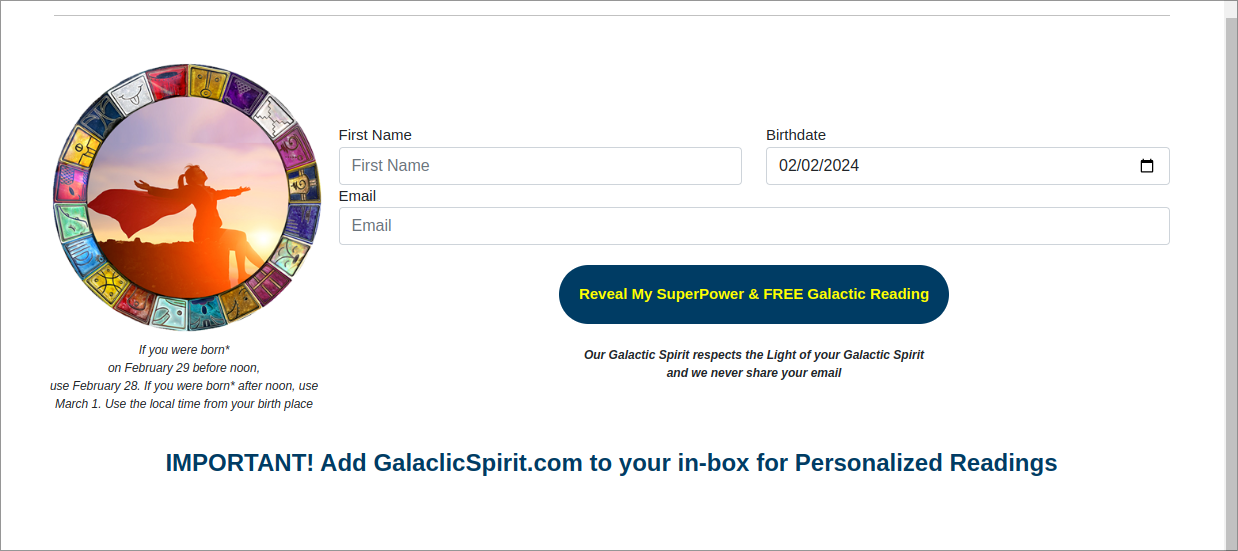
\includegraphics[width=0.45\textwidth]{SinupPage.png}
    \end{center}
  \end{figure}
  \vspace{-2.5em}
  La page d'inscription est diponible depuis la page principale sous l'onglet 
  \texttt{SNGN-IN}. Or, pour s'inscrire, il faut naviguer à travers plusieurs 
  pages pour finalement entrer ses informations personnelles. Nous discuterons 
  des problèmes inhérent à cette approche dans notre critique


%  \begin{figure}[H]
%    \scriptsize{
%   \dirtree{%
%  .1 Barre de navigation $\mathbb{P}$ principale.
%  .2 SIGN-IN.
%  .3 Sélectionner Memberships SIGN-UP. 
%  .4 $\mathbb{P}$ SIGN-UP avec offre de produits.
%  .5 $\dots$ Trouver le lien \textcolor{myb}{Register and Enjoy!}.
%  .6 Vrai page de SIGN-UP.
%  }}
%  \end{figure}

  \section{Page de connexion}
  L'option de connexion est disponible sur la page principale; \textbf{il n'y a pas}  
  de page uniquement consacrée à la connexion. Il faut donc 
  appuyer sur l'onglet SIGN-IN pour entrer ses informations personnelles 
  de compte. 
  \vspace{-2em}

  \section{Page Principale}
  \vspace{-2em}
    \begin{figure}[H]
    \scriptsize{
     \dirtree{%
    .1 Barre de Naviguation.
    .2 E-Learn.
    .3 \entouree{\{ sous-options \}}.
    .4 Law of attaction.
    .5 \entoure{\{ liens \}}.
    .6 \textit{Why doesn't 'Law of Attraction work' }. 
    .6 \textit{Click Here ... Manifestation Mastery E-learn}.
    .4 What is Galactic for.
    .5 \entoure{\{ liens \}}.
    .6 \textit{Why doesn't 'Law of Attraction work' }.
    .4 $\dots$. 
    .4 FREE! Treasure Chest.  
    .5 \entoure{\{ liens \}}.
    .6 \textit{Why doesn't 'Law of Attraction work' }.
    .2 SIGN-UP.
    .3 SIGN-IN. 
    .4 Username.
    .4 Password. 
    .3 \entoure{\{ liens \}}.
    .4 Forgot Password.
    .4 \textit{Join Jami Live On E-Lean}.   
    .2 TODAY's. 
    .3 $\dots$.
    .2 ACTIVATE.
    .3 $\dots$.
    .2 EVOLVE. 
    .3 $\dots$.
    .2 MASTER. 
    .3 $\dots$.
    .2 5D. 
    .3 $\dots$.
    .2 GUIDES. 
    .3 $\dots$.
    .2 STORE. 
    .3 $\dots$.
    }} 
    \caption{Aperçu de la barre de naviguation sur la $\mathbb{P}$. principale}
    \end{figure}


  \begin{note}{}{}
      Chaque \textbf{onglet} de la barre de naviguation comprend 
      au moins 4 \textbf{sous-options} organisées dans une menu défilant.   
  \end{note}


  \section{Page d'activité principale}
  L'organisation du site est trop granulaire pour qu'on puisse identifier 
  une unique \textit{page d'activité principale}. En effet, la quantité 
  oppressante de pages, d'onglets et de liens cliquables nous laissent 
  croire qu'aucune des pages ne constitue une page d'activité principale. 
  La naviguation est volatile; il faut cliquer ici et là, découvrir ceci et 
  cela. 

  En étant plus cynique, on constate que ce choix de design est probablement 
  volontaire. L'idée serait de captiver l'attention  de l'usager le plus 
  longtemps possible, alors qu'il navigue sur toutes les pages 
  et est redigiré à travers tous les liens en esseyant de comprendre 
  quelles options lui sont offertes. 
  
  De plus, chaque page contient un ou plusieurs éléments qui suggèrent 
  qu'on s'inscrive à un service ou achète un produit. Ainsi, le site 
  est essentiellemennt un \textit{grift} : une plateforme feignant 
  d'informer le lecteur sur des pratiques ésothériques et spirituelles 
  \textbf{dans le but ultime de lui faire acheter un produit}.
  
  En considérant ces éléments, nous concluons alors que la 
  \textit{page d'activité principale} est en fait la page de magasinage 
  (STORE) disponible à partir de la page principage.

  \begin{note}{}{}
    La magasin (STORE) est \textbf{divisé en 7 pages} chacune ayant une thématique 
    différente et une panoplies de produits et services. 
  \end{note}


    \begin{figure}[H]
    \scriptsize{
     \dirtree{%
    .1 Barre de Naviguation.
    .2 STORE.
    .3 \entouree{\{ sous-options \}}.
    .4 \textcolor{myb}{Save-Money Bundle (Tools)}. 
    .5 \entoure{\{ liens \}}.
    .6 \textit{Galactic Store}. 
    .6 \textit{Galactic Compass}. 
    .6 \textit{Meditation \& Chakra Crystals}. 
    .4 \textcolor{myb}{Infinity Compass}.  
    .5 \entoure{\{ liens \}}.
    .6 \textit{Explore a LifeTime of DAILY Evolutions}.
    .6 \textit{Click Here to Get Your Compass}.
    .4 $\dots$ \textbf{(Quatre autres options)}  . 
    .4 \textcolor{myb}{E-Learn \& Manifest}.     
    .5 \entoure{\{ liens \}}.
    .6 \textit{Click Here to Get Your Manifestation Mastery E-learn}.
    .6 \textit{Why doesn't 'Law of Attraction work' }.
    }}
    \end{figure}

  \begin{Exercice}{(5 pts)}{}
    Écrivez un \textbf{scénario}, c’est-à-dire une séquence d’actions sur 
    la façon dont vous utiliseriez cette
    interface
  \end{Exercice}


  \section{Persona}
  \textbf{Zephyra} est une jeune ingénieure talentueuse de 23 ans, 
  évoluant dans le monde dynamique du développement de jeux vidéo. 
  Lors d'une conversation détendue avant une réunion d'équipe, 
une de ses collègues lui parle \textit{d'un site Web} récemment découvert.

  \textbf{Améthiste}, une femme accomplie aux portes de la retraite, 
  occupe un rôle clé en tant que gestionnaire des ressources humaines. 
  Zephyra, bien consciente de l'intérêt d'Améthiste pour la spiritualité, 
  les pratiques tantriques, la découverte des chakras et l'astrologie, 
  est elle-même attirée par ces sujets. Cependant, elle est initialement 
  sceptique quant à l'utilité d'un site Web dédié, préférant les sources 
  variées et interactives disponibles sur des plateformes telles que 
  \texttt{TikTok}.

  Soucieuse de tisser des liens amicaux avec sa supérieure et désireuse 
  de combler le fossé générationnel entre elles, Zephyra décide de donner 
  une chance à cette recommandation. À la fin de leur échange, elle exprime 
  à Améthiste sa curiosité grandissante et s'engage à explorer le site 
  pour partager ses impressions.


  \section{Scénarios et cas d'utilisation} 

  \paragraph{Visite initiale}
  Lors de sa première visite, Zephyra est attirée par le 
  \textit{design unique} du 
  site et commence par explorer les différentes \textbf{sections}
  présentées sur la page d'accueil. Elle s'intéresse particulièrement 
  aux \textit{lectures gratuites} marquées par le texte 
  \textcolor{red}{\texttt{FREE!}} et aux informations sur l'ascension, 
  parcourant les titres et les images pour se faire une idée 
  du contenu offert Elle constate rapidement la quantité impressionnante 
  de sections et de liens cliquable et tente de comprendre 
  la \textit{signification} de chacun d'eux.


%  \begin{figure}[H]
%    \begin{center}
%      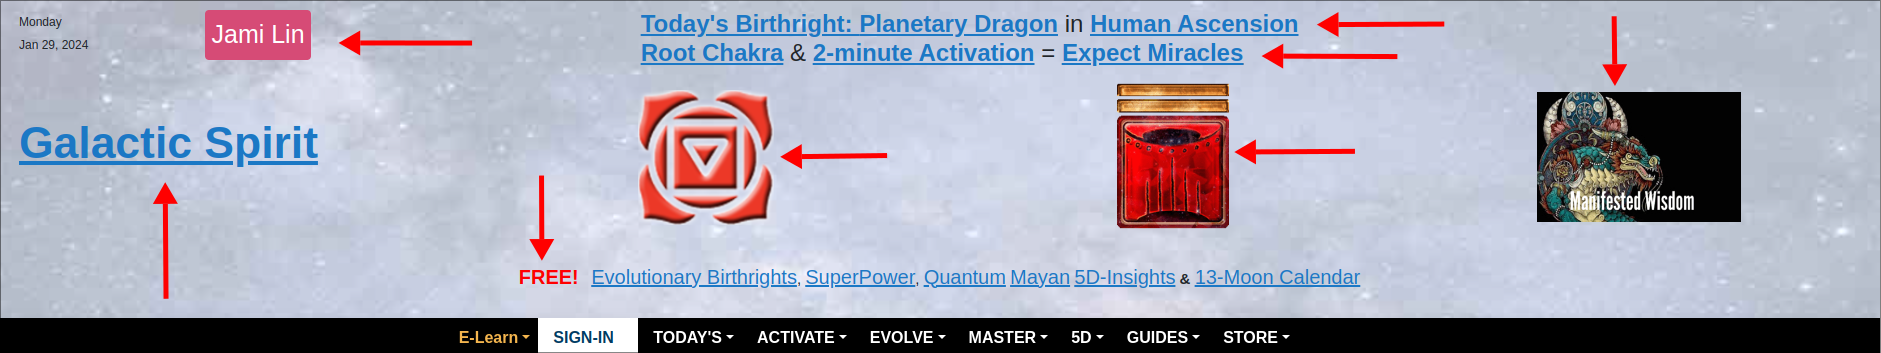
\includegraphics[width=0.45\textwidth]{NavigationInitialeNavbar.png}
%    \end{center}
%  \end{figure}


  \paragraph{Naviguation}
  Zephyra utilise la barre de naviguation pour explorer 
  les différentes catégories du site. Elle clique sur des onglets et 
  sous-menus, découvrant divers services et contenus. 
  Elle passe du temps à examiner chaque section, essayant de 
  comprendre la structure du site et la relation entre les différentes 
  parties.

  \paragraph{Recherche d'information}
  Dans cette étape, 
  Zephyra se concentre sur la collecte d'informations spécifiques. 
  L'auteure du site, \textit{\textit{Jami Lin}}, semble avoir un système  
  compréhensif pour l'épanouissement personnel et l'éveil spirituel. 
  Le site comprend une grande quantité d'information liées à 
  sa \textit{philosophie}. 
  Zephyra clique donc sur des liens pour approfondir sa compréhension des 
  services et  informations, 
  lit des descriptions détaillées et regarde 
  éventuellement des vidéos ou des images associées pour enrichir 
  sa compréhension.




  \paragraph{Inscription}
  Zephyra décide de s'inscrire pour accéder à plus de contenus. Elle 
  remplit le formulaire d'inscription, fournissant ses informations
  personnelles et créant un compte utilisateur. Elle prend le temps de 
  lire les termes et conditions et complète le processus d'inscription.



  \paragraph{Exploration du contenu personalité}
  Une fois inscrite, Zephyra explore les fonctionnalités personnalisées. 
  Elle navigue à travers les options disponibles pour 
  les utilisateurs enregistrés, découvrant des lectures personnalisées, 
  des activations et d'autres contenus exclusifs. Elle teste différentes 
  fonctionnalités pour voir comment elles répondent à ses intérêts.


  \paragraph{Recherche de support et contact}
  Zephyra cherche des informations supplémentaires ou de l'aide sur 
  l'utilisation du site. Elle navigue vers la section d'aide ou de 
  contact, où elle recherche des FAQ, des guides d'utilisation, ou 
  un moyen de contacter directement le support client ou l'auteur \textit{Jami Lin}, 
  puisqu'il est mentionné plusieurs fois qu'il est possible de la 
  contacter directement par courriel. 

  \chapter{Critique}
  \begin{Exercice}{(30 pts)}{}
    Critiquez cette interface à l’aide des \textit{objectifs d’usabilité} et des 
  \textbf{10} \textit{heuristiques d’évaluation}. Écrivez un minimum 
  de \textbf{10} problèmes que vous voyez dans l’un de ces quatre écrans.     
  \end{Exercice}

  \section{Problèmes fondamentaux}

  \subsection{Clarté et raison d'être} 
  Un problème majeur du site de \textit{\textit{Jami Lin}} est le manque de clarté concernant sa 
  raison d'être, ce qui impacte directement les principes d'utilisabilité tels que 
  \textbf{l'utilité} et la compréhension par l'utilisateur. Pour un nouveau visiteur, 
  comprendre l'objectif du site - s'il s'agit d'un blog, d'une plateforme de 
  services électroniques, d'un site communautaire pour les passionnés de spiritualité,
  ou d'une boutique de cristaux - est complexe. Le manque de clarté 
  compromet plusieurs heuristiques 
  de conception d'interface. En effet, l'ambiguité quant à la raison d'être 
  contribue au manque de 
  \textbf{visibilité de l'état du système}, puisque le site ne communique pas 
  clairement son objectif ou ses fonctionnalités principales dès l'entrée sur 
  la page d'acceuil. 
  Il y a également un manque de \textbf{correspondance}; le site ne parvient pas 
  à utiliser un langage ou des conventions qui seraient familiers et compréhensibles 
  par un utilisateur moyen. En effet, à cause du langage ésothérique 
  qu'utilise l'auteure, on a du mal à décrypter pourquoi la plateforme existe 
  et qu'est-ce qu'elle peut offrir. Il faut donc plusieurs visites 
  ou une naviguation prolongée pour se familiariser avec le jargon utilisé. Ce défaut 
  touche également au principe de \textbf{reconnaissance et rappel}. En l'occurence, 
  les uttilisateurs doivent parcourir le site pour assembler des informations 
  disparates \textit{afin de comprendre son but}, plutôt que de reconnaître
  ledit but instantanément. Ainsi, le  site ne rend pas sa \textit{raison d'être} immédiatement 
  claire et cette confusion initiale pourrait entraver l'engagement de 
  l'utilisateur et diminuer la satisfaction globale, affectant ainsi l'expérience 
  utilisateur (UX) dans son ensemble.
  
  \begin{itemize}
    \item [$\rhd$ ] \textbf{Défaut de clarté et raison d'être du site Web}  
      \begin{itemize}
        \item [$\blacktriangleright$ ] $\mathbb{C}$ompréhension du fonctionnement  
        \item [$\blacktriangleright$ ] $\mathbb{U}$tilié 
        \item [$\blacktriangleright$ ] $\mathbb{V}$isibilité de l'état du syst.
        \item [$\blacktriangleright$ ] $\mathbb{C}$orrespondance
        \item [$\blacktriangleright$ ] $\mathbb{R}$econnaisance et rappel
      \end{itemize}
  \end{itemize}

  \subsection{Naviguation}
  Le site souffre également de nombreux défaux de naviguation. En effet, le site 
  semble dépourvu d'une structure de naviguation claire, ce qui affecte la 
  capacité de l'utilisateur à trouver des information spécifiques. Parfois, 
  mêmes les opérations les plus simples semblent inexplicablement difficiles 
  à accomplir, à cause de la naviguation confondante. À titre d'exemple, 
  la seule façon de s'\textit{inscrire}   (\texttt{sign-up}) est de cliquer 
  sur l'onglet de la barre de naviguation de la page principale 
  (  \href{https://galacticspirit.com/home.php}{\texttt{https://galacticspirit.com/home.php}})
  qui porte le nom \texttt{sign-in}.  
  Un menu défilant nous offre ensuite l'option d'inscription. Lorsqu'on 
  clique sur \texttt{Memberships SIGN-UP}, on est rediigé sur la page 
  \href{https://galacticspirit.com/members/signup.php}{\texttt{https://galacticspirit.com/members/signup.php}}. Sur cette nouvelle page, il faut repérer le lien 
  \texttt{Register \& Enjoy!}. Ce lien nous mène à la page 
  \href{https://galacticspirit.com/members/free_superpower.php}{\texttt{https://galacticspirit.com/members/free\_superpower.php}}. C'est finalement sur cette page 
  qu'on peut entrer ses informations personnelles pour l'inscription. Cet exemple 
  reflète un problème flagrant au niveau des \textbf{signifiants}. D'une part, on en 
  vient à se demander : pourquoi faut-il cliquer sur un  buton 
  \texttt{SIGN-IN} alors que notre objectif est de \texttt{SIGN-UP} ? 
  D'autre part, on se questionne également quant 
  à la motivation dernière l'idée de forcer le visiteur à naviguer à travers plusieurs 
  pages pour s'inscrire. De plus, on peine à comprendre pourquoi 
  les fonctionnalités d'\textit{inscription} et de \textit{connexion} 
  ne possèdent pas 
  leur propre page dédiée et ne sont pas visibles via des signifiants clairs.\  Finalement, 
  l'absence de \textbf{prévention d'erreur} est indicative de la structure 
  complexe et contre intuitive affectant la naviguation. En effet, plusieurs 
  affordances sont cachées, les signifiants sont contradictoires et les 
  \textbf{correspondances} sont nébuleuses. 
  Ces problèmes de naviguation peuvent conduire à une expérience utilisateur frustrante, 
  diminuant la probabilité de retour sur le site et affectant l'impression générale de 
  l'utilisateur sur la plateforme.


    \begin{itemize}
    \item [$\rhd$ ] \textbf{Défauts de Naviguation}  
      \begin{itemize}
        \item [$\blacktriangleright$ ] $\mathbb{A}$ffordances difficle d'accès 
        \item [$\blacktriangleright$ ] $\mathbb{S}$ignifiants contradictoires
        \item [$\blacktriangleright$ ] $\mathbb{P}$révention d'erreurs lacunaire
        \item [$\blacktriangleright$ ] $\mathbb{C}$orrespondance nébuleuse
      \end{itemize}
  \end{itemize}

  \section{Problèmes esthétiques}
  \subsection{Présentation du contenu}
  Sur l'entièreté du site, la présentation du contenu est 
  inutilement dense. Et contrairement à certains média 
  à travers lesquels la densité d'information est un choix délibéré 
  (articles scientifiques, journaux, blogs techniques, etc.) cette décision 
  de design ne remplit aucune \textbf{utilité}. Au contraire, elle 
  tend à confondre le lecteur, qui est alors submergé par l'excès 
  d'information 
  de choix et de liens cliquables. La \textbf{page principale} est particulièrement 
  affectée par ce défaut. Sur celle-ci, on retrouve des images 
  non pertientes; des liens vers les 
  \textit{entraînements d'activation de droit de naissances};  
  des liens vers les \textit{entraînements d'activation de chakra};
  des liens vers les \textit{entraînement de création quantique}; 
  des liens vers les \textit{entraînements de méditation}; des informations 
  sur la \textit{création quantique}; une vidéo d'introduction 
  à la philosophie \textit{Galactic Spirit} de \textit{\textit{Jami Lin}}; 
  des informations sur l'attraction magnétique, et plus encore. 
  Ainsi, le site enfreint l'heuristique de 
  \textbf{design esthétique et minimaliste}, puisque l'utilisateur 
  est confronté à un encombrement visuel qui nuit à la clarté. 
  La façon dont le contenu est présenté nuit également 
  à la \textbf{prévention des erreurs}, puisque la densité 
  excessive d'nformation et de choix conduit à des erreurs de naviguation 
  où, par exemple, l'utiliateur clique accidentellement sur des 
  liens inappropriés. Finalement, le choix de design viole l'heuristique de 
  \textbf{reconnaissance plutôt que rappel}. En effet, la surchage 
  d'information rend difficile pour l'utilisateur de se rappeler 
  où trouver des éléments spécifiques du site. 


  \begin{itemize}
    \item [$\rhd$ ] \textbf{Défauts de présentation du contenu}  
      \begin{itemize}
        \item [$\blacktriangleright$ ] $\mathbb{U}$tilié des différents éléments 
        \item [$\blacktriangleright$ ] $\mathbb{D}$esign esthétique et minimaliste 
        \item [$\blacktriangleright$ ] $\mathbb{P}$révention d'erreurs lacunaire
        \item [$\blacktriangleright$ ] $\mathbb{R}$econnaisance et rappel
      \end{itemize}
  \end{itemize}
  \vspace{-1em}


  \subsection{Choix esthétiques}
  Plusieurs problèmes de ce site sont dus aux choix esthétiques. 
  Par exemple, les images ne sont pas évocatives. Pour ceux qui ne sont pas 
  initié à la philosophie de \textit{\textit{Jami Lin}}, il est difficle de 
  déterminer si chacune des images sur la \textbf{page principale} a un signification 
  particulière ou si elles ont été choisies au hasard. Par exemple, 
  les quatres images qui accompagnent les liens vers les pages 
  \texttt{Evolve Best Version Of YOU}; \texttt{Reclaim Your SuperPower}; 
  \texttt{Awaken Galatic Ascensions} et \texttt{Master Your Quantum Self} sont 
  similaires mais présentent de légère variantes. Quelle est la pertinence 
  de ses variantes ?
  Que représente chacun des symboles sur l'image ? Pourquoi les mêmes 
  symboles sont présentés alors qu'il s'agit de \textit{différents programmes} ?   
  \begin{figure}[H]
    \begin{center}
      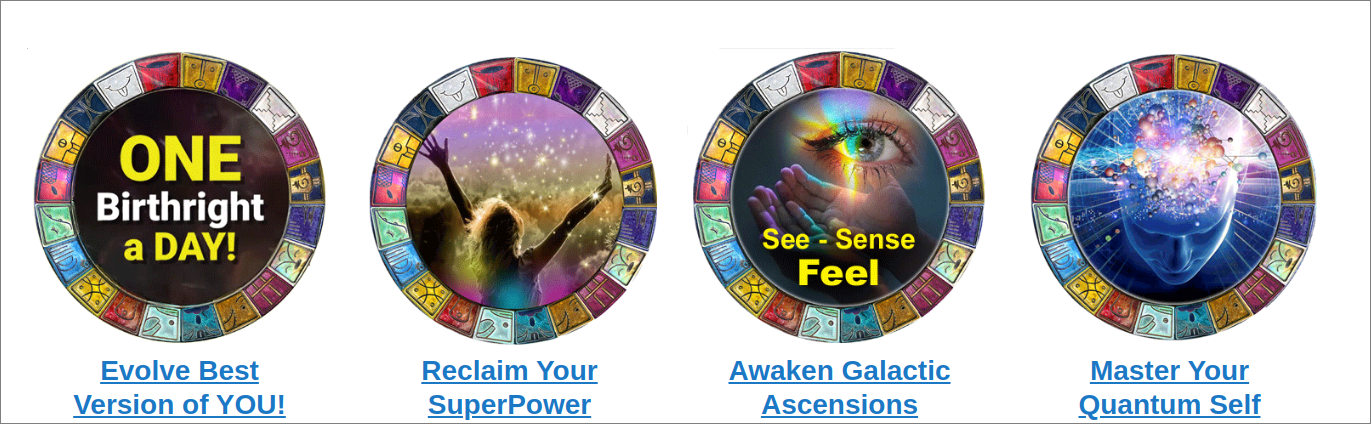
\includegraphics[width=0.35\textwidth]{ImagesConfondantes.png}
    \end{center}
    \caption{Sélection d'images sur la page principale}
  \end{figure}

  Pour ceux qui n'y sont pas initié, certaines images parraissent 
  cryptiques; la plupart des nouveaux utilisateurs ne pourraient pas 
  déterminer leur sens ou leur raison d'être. 

  \begin{figure}[H]
    \begin{center}
      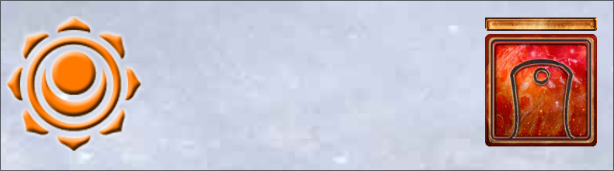
\includegraphics[width=0.25\textwidth]{ImageConfondantes2.png}
    \end{center}
    \vspace{-1em}
    \caption{Images de symboles cryptiques sur la page principale}
  \end{figure}

  Par ailleurs, on constate à travers les différentes pages 
  des choix esthétiques qui ne semblent pas avoir de fonction utiliaire. 
  Par exemple, certains liens sont soulignés et d'autres ne le sont pas; 
  certains liens ont une couleur bleu foncée, d'autres ont une couleur bleu pâle; 
  certaines portions de texte sont surligné avec un couleur jaune, d'autres ne le sont pas; 
  certaines informations sont encadrées (sans qu'elles semblent avoir une importance 
  particulières) et certaines informations qui semblent importante sont présentées 
  directement sur la page; différentes taille de police de caractère sont utilisées 
  alors qu'aucune  attention n'est porté quant à la hiérarchie 
  ou l'importance relative des éléments. Ainsi, 
  Les images cryptiques et les choix de \textbf{design inconsistants}
  exigent que les utilisateurs
  dépensent plus d'effort pour comprendre le contenu, ce qui n'est pas 
  idéal pour une \textbf{reconnaissance} facile. Et il va 
  sans dire que  l'incohérence dans le style des liens, la couleur du texte, 
  et les surlignages peut dérouter les utilisateurs, 
  enfreignant ce principe de conception.

  \begin{itemize}
    \item [$\rhd$ ] \textbf{Défauts de choix esthétiques}  
      \begin{itemize}
        \item [$\blacktriangleright$ ] $\mathbb{U}$tilié des différents éléments 
        \item [$\blacktriangleright$ ] $\mathbb{D}$esign esthétique et minimaliste 
        \item [$\blacktriangleright$ ] $\mathbb{P}$révention d'erreurs lacunaire
        \item [$\blacktriangleright$ ] $\mathbb{C}$ohérences et normes
      \end{itemize}
  \end{itemize}


  \subsection{Consistance des éléments visuels}
  Le site souffre d'un manque de consistance en ce qui a trait des 
  éléments visuels. Ce problème est étroitement lié à celui des choix 
  esthétiques. En effet, le manque de consistance transparait dans les 
  choix de couleurs, les choix de polices de caractères et de taille 
  de la police de caractère, ainsi qu'à travers 
  l'utilisation d'images et l'utilisation d'éléments structurants, 
  et plus encore. Ansi, 
  le manque de consistance affecte l'expérience utilisateur en termes 
  de \textbf{reconnaissance}. L'utilisateur doit constamment s'adapter à 
  la nouvelle convention utilisée pour l'affichage d'un élément et ce, 
  pour la totalité des pages présentes sur le site. Pourquoi  
  trouvons-nous des blocs de texte ayant une couleur de fond jaune 
  sur la \textbf{page principale} ? Est-ce que cet élément est plus important que 
  les autres ? Pourquoi le bouton jaune \texttt{Free Memberships} apparaît 
  sur la \textbf{page principale} deux fois, alors que sur cette même page 
  on y trouve également 
  un lien souligné en bleu portant le nom \texttt{Get Your Free Password} ?   
  Ces liens mènent-ils à la même page ? Si oui, pourquoi ces 
  trois affordances sont-elles présentées à trois endroits différents 
  sur la même page sans consistance ? Qu'est-ce qu'un 
  \textit{mot de passe gratuit} ? Ce dernier questionnement soulève 
  un défaut associé à l'heuristique de \textbf{cohérence et normes}.
  Un utilisateur moyen est familier avec le concept \textit{d'abonnement gratuit}  
  et le language utilisé pour faire référence à cette fonctionnalité 
  est généralement évident sur la plupart des plateformes. 
  Or, l'expression \textit{mot de passe gratuit} 
  est une formulation non conventionnelle pour désigner un abonnement 
  libre de frais. 

  \begin{itemize}
    \item [$\rhd$ ] \textbf{Défauts de consistance des éléments visuels}  
      \begin{itemize}
        \item [$\blacktriangleright$ ] $\mathbb{C}$ohérence et normes
        \item [$\blacktriangleright$ ] $\mathbb{R}$econnaisance plutôt que rappel 
        \item [$\blacktriangleright$ ] $\mathbb{D}$esign esthétique et minimaliste 
      \end{itemize}
  \end{itemize}
  

  \subsection{Accessibilité}
  Les défauts esthétiques tendent à réduire l'accessibilité du site 
  pour certains usagers. À titre d'exemple, la taille de la police de 
  caractère et la couleur de celle-ci 
  rend le texte pratiquement illisibile pour certaines 
  sections de la \textbf{page principale} ainsi que de la page d'inscription 
  \begin{figure}[H]
    \begin{center}
      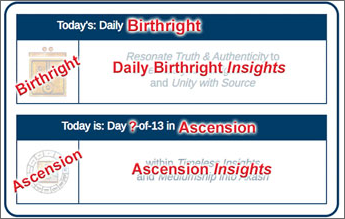
\includegraphics[width=0.15\textwidth]{PoliceIllisible.png}
    \end{center}
    \vspace{-1em}
    \caption{Section de la page principale difficile à lire}
  \end{figure}
  Par ailleurs, certaines portions sont excessivement coloré sans que 
  les choix de couleur aient une utilité ou une \textbf{correspodance}
  avec les conventions normalemett utilisées. Les contrastes choisit 
  engendrent également des problème d'accessibilité. Dans l'ensemble, 
  de nombreux choix esthétiques rendent le site moins accessible et 
  risque de réduire l'expérience des utilisateurs ayant une 
  invalidité visuelle. 
  \begin{itemize}
    \item [$\rhd$ ] \textbf{Défauts d'accessibilité}  
      \begin{itemize}
        \item [$\blacktriangleright$ ] $\mathbb{V}$isibilité
        \item [$\blacktriangleright$ ] $\mathbb{E}$fficience réduite
      \end{itemize}
  \end{itemize}


  \section{Expérience utilisateur}

  \subsection{Orientation de l'utilisateur}
    Il semble y avoir un manque d'orientation  
    et de \textbf{signifiants} permettant de guider les utilisateurs 
    lors de la naviguation sur le site. Par exemple, sur la 
    page principale on retrouve ce qui s'apparente à un 
    \textit{guide d'utilisation} du site pour les utilisateurs 
    voulant s'abonner. Or, cette section de la  
    \textbf{page principale}  souffre des même problèmes
    que les autres portions du site. Il y a un excès d'information 
    qui est non seulement déroutant mais risque 
    par ailleurs d'affecter \textbf{l'efficience}  
    des nouveaux usagers tentant d'appréhender la plateforme.

  \begin{figure}[H]
    \begin{center}
      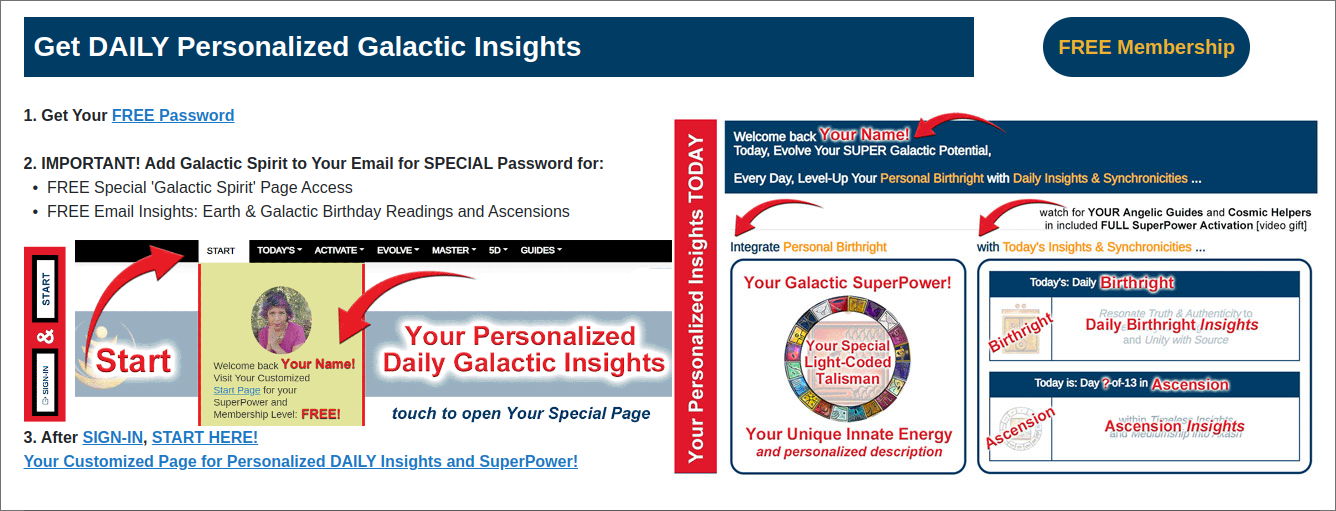
\includegraphics[width=0.45\textwidth]{Orientation.png}
    \end{center}
    \caption{Guide de commencement présent sur la page principale}
  \end{figure}

    Par conséquent, on observe que le principe de \textbf{visibilité} 
    est enfreint. En effet, dans cette section il n'est pas 
    évident pour un utilisateur quelle séquence de contrôle est 
    nécessaire pour atteindre son but, puisque l'information 
    n'est pas présentée de façon intuitive. 
    Par ailleurs, Cette section 
    encapsule également les défauts esthétiques et les 
    lacunes de consistance mentionnés plus tôt. Finalement, plusieurs 
    \textbf{signifiants} de cette section sont redondants, 
    lorsqu'ils ne sont pas carrément contradictoires ou 
    contre-intuitifs. Quelle est la différence entre 
  \texttt{Your Customized Page for Personalized DAILY insights and SuperPower!}  et \texttt{Your Personalized Insights TODAY} ? Quelle est la différence 
  entre \texttt{Your Galactic SuperPower!} et \texttt{Your Special Light-Colored Talisman} et \texttt{Your Unique Innate Energy \textit{and personalized description}} ? À quoi servent chacun de ces services ? Vers quels éléments 
  les flèchent rouges poitent-elles ? Quel est leur but : nous orienter 
  dans la naviguation, pointer vers les éléments les plus importants 
  ou simplement captiver l'attention du lecteur sans véhiculer de 
  signification particulière ? Ainsi, l'orientation des utilisateurs 
  est sévèrement lacunaire. Et malgré les tentatives visant à guider les usagers à travers la naviguation, les informations présentées 
  sont redondantes, contradictoires ou contre-intuitives. 


  
  \begin{itemize}
    \item [$\rhd$ ] \textbf{Défauts de d'orientation de l'utilisateur}  
      \begin{itemize}
        \item [$\blacktriangleright$ ] $\mathbb{S}$gnifiants incohérents
        \item [$\blacktriangleright$ ] $\mathbb{E}$fficience réduite
        \item [$\blacktriangleright$ ] $\mathbb{V}$isibilité lacunaire 
      \end{itemize}
  \end{itemize}

  \subsection{Engagement des utilisateurs}
  Les stratégies utilisées pour engager les utilisateurs pourraient 
  être améliorées, afin d'obtenir une meilleure rétention. Une des  
  principales stratégies de rétention utilisée par \textit{\textit{Jami Lin}} 
  est la mise en évidence des services et fonctionnalités gratuites. 
  En effet, on voit souvent le message \texttt{\textcolor{red}{FREE}} 
  partout à travers le site. Or, l'annoncement des services gratuits 
  offerts est répété et disponible à travers plusieurs éléments. Parfois, 
  un simple texte annonce le service gratuit; parfois l'annoncement 
  se retrouve dans un menu défilant; et parfois l'annoncement se trouve 
  dans la barre de naviguation ou encore à travers un lien cliquable nous 
  redirigeant vers une autre page. Cette approche 
  contribue à la surcharge d'information et tend à rendre 
  l'expérience de l'utilisateur frsutrantre, puisqu'il doit 
  déchiffrer et interpréter des \textbf{signifiants}  redodants. 


  \begin{itemize}
    \item [$\rhd$ ] \textbf{Défauts d'engagement des utilisateurs}  
      \begin{itemize}
        \item [$\blacktriangleright$ ] $\mathbb{S}$gnifiants redondants
        \item [$\blacktriangleright$ ] $\mathbb{E}$fficience réduite
      \end{itemize}
  \end{itemize}

  \subsection{Rhétorique et pertinence du message}
  À travers le site, l'information véhiculée est rarement immédiatement 
  évidente. Indépendamment de la véracité de ses propositions
  \textit{\textit{Jami Lin}}  a tendance à \textit{affirmer} sans pour 
  autant \textit{expliquer}. Le manque d'explication, l'utilisation 
  jargon impénétrable et la nature cryptique et esothérique 
  des sujets abordés rendent l'information indigeste pour les nouveaux 
  utilisateurs. 
  \begin{figure}[H]
    \begin{center}
      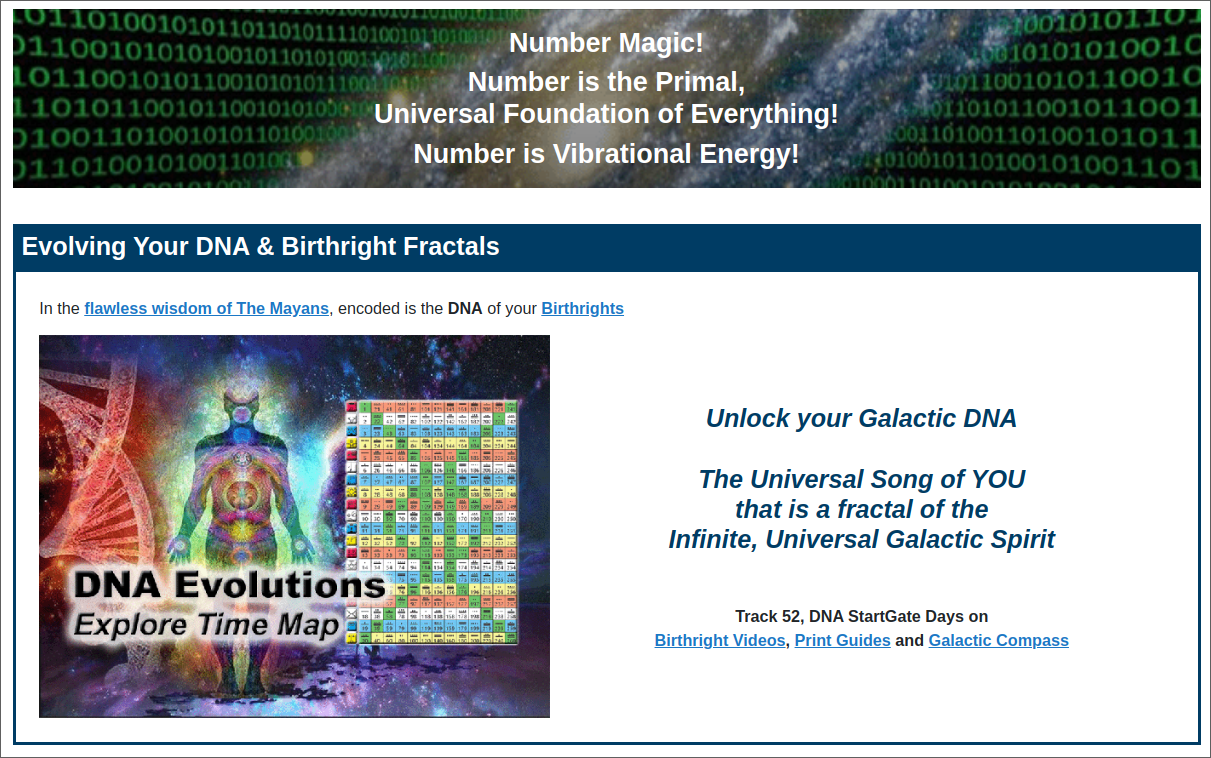
\includegraphics[width=0.35\textwidth]{PertinenceMessage.png}
    \end{center}
    \caption{Exemple de concepts inaccessibles}
  \end{figure} 
  À titre d'exemple, un utilisateur nivaguant sur le site pourrait 
  se poser les question suivantes : 
  \begin{itemize}
    \item Qu'est-ce qui fait en sorte que les nombres sont \textit{magiques} ?   
    \item Qu'est-ce qui rend un nombre \textit{primal} et qu'est-ce 
      que la primauté, selon \textit{\textit{Jami Lin}} ?
    \item Quelle est la connexion entre les nombres et l'énergie vibrationnelle?
    \item Qu'est-ce que l'énergie vibrationnelle, selon \textit{\textit{Jami Lin}} ?  
    \item Qu'est-ce qu'un ADN galactique ?
    \item Qu'est-ce qu'un fractal de \textit{l'infini et universel esprit galactique} ?  
  \end{itemize}

  Le plus gros défaut de \textit{\textit{Jami Lin}} n'est donc pas 
  l'inacessiblité de son message, mais plutôt le manque 
  de rhétorique persuasive qui permettrait autrement de 
  rendre l'incohérence de son message passablement digeste. Cette 
  lacune viole donc le principe \textbf{d'utilité}; l'utilisateur 
  ne sait pas que faire de l'information et n'a aucun repère 
  quant aux modèles du monde réel avec lequels il pourrait 
  établir une correspondance. 

  \begin{itemize}
    \item [$\rhd$ ] \textbf{Défauts de rhétorique et pertinence du message}  
      \begin{itemize}
        \item [$\blacktriangleright$ ] $\mathbb{U}$tilié
        \item [$\blacktriangleright$ ] $\mathbb{C}$orrespondance entre le système et le monde réel
      \end{itemize}
  \end{itemize}

  \subsection{Surchage et organisation de l'information} 
  Les problèmes fondamentaux, les problèmes esthétiques et 
  les problèmes d'expériences utilisateur sont tous 
  liés à la surchage d'information.  Et par conséquent, la 
  \textbf{découvrabilité} est sévèrement affectée. 
  Les \textbf{affordances} sont souvent cachées et manquent 
  de signifiants clairs. Le site manque également de 
  \textbf{contraintes} pour restreindre la naviguation et 
  offrir un flux intuitif pour aller d'une page à une autre. Parce qu'il 
  y a une surchage d'information, le principe de \textbf{feedback} est 
  également négligé. En effet, au lieu d'indiquer clairement 
  l'effet d'une action lorsqu'on clique sur un lien, on 
  se retrouve généralement sur une autre page contenant 
  une davantage de liens cliquables. Ainsi, le défaut de surchage 
  d'information affecte considérablement la découvrabilité 
  du site et rend l'expérience utilisateur pénible en termes de 
  naviguation. 


  \begin{itemize}
    \item [$\rhd$ ] \textbf{Défauts de surcharge de l'information}  
      \begin{itemize}
        \item [$\blacktriangleright$ ] $\mathbb{D}$édécouvrabilité difficile
        \item [$\blacktriangleright$ ] $\mathbb{F}$eedback lacunaire
      \end{itemize}
  \end{itemize}

  \chapter{Correction}

  \begin{Exercice}{(30 pts)}{}
     Pour chacun des problèmes rencontrés, proposez une solution concrète. 
     Justifiez pourquoi cette solution est meilleure. Utilisez, 
     quand possible et nécessaire, la terminologie qu’on a appris dans 
     le cours.     
  \end{Exercice}

  \paragraph{Clarté et raison d'être}
Premièrement, il faut indiquer le but du site dès la page d’accueil. En s’assurant que les utilisateurs comprennent immédiatement ce que propose le site. Cela peut être réalisé en utilisant un texte d’introduction clair et concis qui mets en relief le but du site, ses fonctionnalités principales et les services qu’il offre.
Deuxièmement, il faut utiliser un langage approprié et accéssible. En évitant d’utiliser un langage ésotérique qui s’avérera déstabilisant pour un nouvel utilisateur.
Finalement, il faut s’assurer que l’utilisateur n'éprouve pas de difficulté à chercher l’information dont il a besoin. Pour cela, une structure de naviguation claire et une organisation du contenu de manière logique sont nécessaires.
En adoptant ces solutions, la visibilité de l’état du système est mise en évidence, ce qui tend à aider l’utilisateur à comprendre son l'objectif et les fonctionnalités principales dès l’entrée sur la page d’accueil.

  \paragraph{Naviguation}
Il faut agrandir les signifiants et les rendre plus facile à identifier et utiliser. Ainsi, il serait plus facile pour l’utilisateur de profiter des affordances du site web. Également, le risque d’erreur est diminué puisqu’il est plus facile de cliquer sur les signifiants.

  \paragraph{Présentation du contenu}
Il faut éviter de submerger l’utilisateur d'informations, de choix et de liens cliquable. Pour remédier a cette problématique, il serait judicieux de réduire le nombre d’information présenté sur la page principale et éliminer les informations inutiles.
Il faut ainsi opter pour une 
conception minimaliste qui rendrait la page d’accueil plus épurée.

\paragraph{Choix esthétique}
Une clarification de la signification des images est primordiale. Les utilisateurs qui ne sont pas initié à la philosophie de \textit{\textit{Jami Lin}} ont du mal à comprendre le sens des figures et images présentées. Pour cela, il serait judicieux d’ajouter une légende et une description à l’image, lorsque nécessaire.Autrement, il faut s'assurer que les images choisie soit suffisamment évocatrice et que leur usage ne nécessite pas l'ajout d'une légende. 

\paragraph{Consitance des éléments visuels}
Il faut établir des conventions visuelles cohérentes, en définissant des règles claires pour l’utilisation des couleurs (par exemple utiliser une couler rouge en ce qui concerne une erreur), des tailles de police (par exemple une grande police pour le titre), des styles de texte et des éléments structurants à travers tout le site.
Après avoir adopté ces solutions, l’expérience de l’utilisateur est optimisée puisque le site serait alors cohérent et normé.


\paragraph{Engagement des utilisateurs}
Le site contient beaucoup de signifiants redondents. Ce problème affecte grandement l’efficience pour un utilisateur qui cherche simplement à comprendre le message de \textit{Jami Lin}. On est très souvent distrait par des offres de services gratuit. Une bonne application du principe d’affordance pourrait aider à résoudre ce problème. En suprimmant les signifiants redondants, la présentation du site sera plus rationnelle et réduira le besoin de décoder la signification de chaque offre. En favorisant le principe d’affordance, l’utilisateur passera moins de temps à essayer de naviguer et plus de temps à suivre le message de \textit{Jami Lin}. Le site a tendance également à ouvrir de nouvelles pages quand l’utilisateur clique sur certains liens. Ce changement crée une confusion parce qu’il n’est pas intuitif. Le principe de correspondance exige d’éviter les surprises et les comportements inattendu donc rester sur la même serait un choix préférable pour permettre à l’utilisateur de développer une intuition pour le site.

\paragraph{Rhétorique et pertinence du message}
Supposons que les principales méthodes pour devenir un "Galactic spirit" sont les liens Evolves Best version of You! Reclaim your SuperPower Awaken Galactic Ascensions Master your Quantum Self. Et supposons que cela est relié 
à la motivation personnelle, la santé mentale, etc. Certaines définitions sont présentées le site, mais puisque celui-ci est saturé d’informations il est très difficile de comprendre les mots et les objectifs des leçons de \textit{\textit{Jami Lin}}. Une page expliquant l’expérience personnelle de \textit{\textit{Jami Lin}} avant et après son éveil spirituel aiderait beaucoup à comprendre la pertinence de son message. Il serait intéressant de savoir comment toutes les méthodes qu’elle recommande lui ont servi. Un utilisateur pourrait alors être tenté 
par l'idée de reproduir ses choix de vie. Un bouton \textit{About} pourrait mener vers cette page. Cette solution etablira une correspondance  emotionnelle et pratique entre l’utilisateur le message de \textit{\textit{Jami Lin}}.

\begin{EExample}{}{}
  \href{ https://sophiapersephone.com/sophia-persephone-ambrose/}{ https://sophiapersephone.com/sophia-persephone-ambrose/}
\end{EExample}


\paragraph{Surcharge et organisation de l’information}
Le problème de surcharge d’information pourrait être corrigé en épurant la page d’accueil. La section en dessous de la barre de naviguation jusqu’à get Daily Personalized Galactic insights peut être supprimée. La très grande majorité de ces informations sont déjà présente ailleurs dans le site. La correspondance implique un design intuitif ce qui comprend la mise en évidence des éléments clés du site. La présence de ces informations nuit à ce but et augmente l’effort nécessaire pour utiliser le site.



\paragraph{Orientation de l’utilisateur}
Certains menus contiennent des liens vers des vidéos. Or, une vidéo n’est également pas présente si l’utilisateur clique sur le lien en dessous de la vidéo. Cette approche nuit l’efficience et la satisfaction de l’usager. Toutes les vidéos dans les sous-menus devraient être supprimées ou déplacées vers le lien en dessous des vidéos. La suppression des vidéos permetrait de réduire la surcharge de signifiants général du site et sera plus intuitif puisque des vidéos jouables dans un sous-menu ne suivent pas de normes conventionnel d’affordance. 

\paragraph{Accessibilité}
Le site est parfois difficile à lire. Une solution serait de changer la couleur des éléments textuels et d'agrandir les caractères. Il faut 
également éviter l'utilisation de fonds rouges jumelées à une police de 
caractères blanche. Il serait judicieux de choisir des couleurs plus sombres. Une visibilité claire et intuitive est primordiale dans le principe de correspondance. L'apparance du site serait alors plus abordable, ce qui tend 
à réduire les frustrations pour l’utilisateur.

\begin{Exercice}{(30 pts)}{}
 Implémentez les quatre écrans avec vos corrections en tant que prototype Figma. Assurez-vous
que le prototype est fonctionnel : il doit réagir à toutes les interactions nécessaires pour montrer les
problèmes que vous résolvez. Assurez-vous que l’utilisateur peut naviguer les écrans en cliquant
sur les boutons nécessaires. L’implémentation de fonctionnalités qui ne sont pas couvertes par votre
scénario et vos problèmes n’est pas nécessaire.
La conception graphique ne sera pas évaluée à moins qu’elle n’interfère avec l’utilisabilité.   
\end{Exercice}

\begin{center}
  $\Big|$ \href{https://www.figma.com/proto/ljLKsuKg3fSQsX0puWfWj6/Galactic_Spiritv4?page-id=0%3A1&node-id=2-1062&starting-point-node-id=1%3A32&t=gDC3pM3wJifRLpeM-1&mode=design}{\textcolor{myb}{Lien vers le prototype Figma}} $\Big|$ 
 
\end{center}

\end{multicols*}
\end{document}
